\documentclass{article}
\usepackage[utf8]{inputenc}
\usepackage[OT2,T2A,T1]{fontenc}
\usepackage[german]{babel}
\usepackage[pdftex]{graphicx}
\usepackage{amsmath}
\usepackage{chngcntr}
\usepackage[vflt]{floatflt}
\usepackage{geometry}
\usepackage{hyperref}
\usepackage{makeidx}
\usepackage{tabularx}
\usepackage{tikz}
\usepackage{url}


\bibliographystyle{unsrt}
\hyphenation{words}
\pagestyle{headings}
\geometry{left=20mm,right=15mm, top=20mm, bottom=20mm}


\title{Dokumentation zum Semesterprojekt Programmierbare Logik: Realisierung des Videospiels "Pong"}
\author{Marc Ludwig, Matthias Springstein}
\date{\today}

\makeindex
\begin{document}

\maketitle
\newpage

\tableofcontents
\newpage

\section{Aufgabenstellung}
\index{Aufgabenstellung}
Ziel des Semesterprojektes ist es, auf dem Entwicklungsboard DE2-70 von Terasic 
\footnote{http://www.altera.com/education/univ/materials/boards/de2-70/unv-de2-70-board.html}
eine Umsetzung des 1972 ertsmals von Atari veröffentlichten Spiels Pong zu implementieren.

Das 1972 von Atari veröffentlichte Pong wurde zum ersten weltweit populären Videospiel und in den 
1970er-Jahren zunächst auf Geräten in Spielhallen bekannt. Es gilt als Urvater der Videospiele, 
obgleich schon zuvor Videospiele entwickelt worden waren.\footnote{http://de.wikipedia.org/wiki/Pong}

Das Spielprinzip von Pong ist simpel und ähnelt dem des Tischtennis: Ein Punkt (Ball) bewegt sich 
auf dem Bildschirm hin und her. Jeder der beiden Spieler steuert einen senkrechten Strich 
(Schläger), den er mit einem Drehknopf (Paddle) nach oben und unten verschieben kann. Lässt man 
den Ball am Schläger vorbei, erhält der Gegner einen Punkt.


\subsection{Anforderungen}
\index{Anforderungen}
\begin{itemize}
  \item durchgeführte Dokumentation des Projektes (Quellcode und Aufgabenbearbeitung)
  	\begin{itemize} 
  	\item Quellcode durch Doxygen 
  		\footnote{http://www.doxygen.org} 
  		\footnote{http://de.wikipedia.org/wiki/Doxygen}
  	\item Aufgabenbearbeitung durch ein PDF Dokument
  		\footnote{http://www.latex-project.org/}
  		\footnote{http://de.wikipedia.org/wiki/LaTeX}
  	\end{itemize} 
  \item funktionale Bedienelemente für beide Spieler
  \item graphische Darstellung auf einem via VGA angeschloßenen CRT/TFT Monitor
  \item Quellcode, basierend auf einem durch mehrere Mitarbeitende Personen realisierbarem Konzept, 
  		welcher kommentiert und dokumentiert ist
\end{itemize}


\section{Dokumentation}
\index{Dokumentation}
Die Dokumentation des Semesterprojektes wird mit dem bereits erwähnten Textsatzsystem LaTeX
durchgeführt und als generierte PDF Datei zur Verfügung gestellt. Eingebundene Abbildungen und 
Diagramme sind ebenfalls im Dokumentationsverzeichnis enthalten.
Die mittels Doxygen erstellte Quellcode Dokumentation liegt als HTML-Dokument 
\footnote{\href{}{LINK ZUR DATEI EINFÜGEN}} vor.


\section{Entwicklunghierarchie}
\index{Entwicklunghierarchie}
Als Entwicklungsansatz wurde zunächst das Top-Down Modell gewählt, unter dem Aspekt, mit einem
spätere Bottom-Up Modell den gewählten Ansatz zu verifizieren. Als zu bevorzugendes Entwurfsmuster
für VHDL Designs ist das Register Transfer Level (im folgenden RTL) gewählt worden.

Charakteristisch für eine RTL-Beschreibung ist die Trennung von Registern und kombinatorischen
Logikstufen, die jeweils das Eingangssignal der nachfolgenden Registerstufe definieren. Vgl. Abb.
\ref{fig:RTL-Logic} Der Datenpfad wird somit als Pipeline aufgefasst. Entsprechend sollen beim reinen RTL-Entwurfsstil 
kombinatorische und getaktete Prozeße streng voneinander getrennt werden.

\begin{figure}[here]
	\begin{center}
		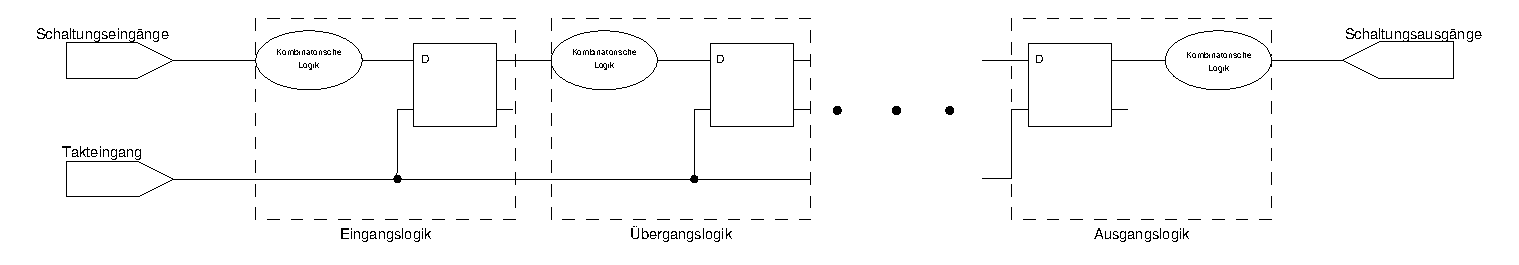
\includegraphics[width=0.65 \textwidth]{includes/RTL-Logic.eps}
		\caption[Darstellung RTL]{Register Transfer Level}
		\label{fig:RTL-Logic}
	\end{center}
\end{figure}

\newpage
\section{Entwicklungsstrategie}
\index{Entwicklungsstrategie}
Bezugnehmend auf dem Daten-Steuerpfad Modell \cite{Reichardt}, 
haben wir uns für folgende Methoden zur Systempartitionierung entschieden.

\begin{itemize}
  \item Hierarchische Strukturierung des Entwurfs
  \item Lokalität der Module und Signale
  \item Reguläre Strukturen
\end{itemize}

\subsection{Hierarchische Strukturierung des Entwurfs}
\index{Methoden zur Systempartitionierung}
Unter Hierarchischer Strukturierung versteht man die Partitionierung einer komplexen Entwurfsaufgabe
in Teilaufgaben sowie deren weitere Gliederung in noch kleinere Einheiten, solange bis die 
Teilprobleme mit einfachen Lösungsansätzen zu beschreiben sind. Mit Hilfe von Komponenten 
(\emph{component}) läßt sich eine hierarchische Problemlösung erreichen. Ergebnis der Synthese ist
letzlich eine hierarchische Netzliste.

\subsection{Lokalität der Module und Signale}
\index{Methoden zur Systempartitionierung}
Dies ist eine Forderung, daß die einzelnen Module zur Lösung der Teilprobleme keine Seiteneffekte
auf benachtbarte Schaltungsteile aufweisen. Durch Blöcke (\emph{block}) lassen sich innerhalb einer
Architektur nebenläufige Anweisungen zu Funktionsblöcken zusammenfassen. Innerhalb von Blöcken 
können lokale Signale definiert werden, die nur innerhalb des Blocks gültig sind.

\subsection{Reguläre Strukturen}
\index{Methoden zur Systempartitionierung}
Dies bedeutet die Verwendung möglichst einheitlich aufgebauter Bibliothekskomponenten. Derartig
reguläre Entwürfe sind einfacher zu beschreiben und zu verifizieren. Prozeduren (\emph{procedure})
und Funktionen (\emph{function}), die insbesondere auch in übergeordneten Bibliotheken 
(\emph{library}) oder Design-spezifischen Bibliotheken (\emph{package}) abgelegt werden können,
dienen dazu, standardisierte Lösungen für häufig auftretende Probleme zu verwenden.

\vspace{10mm}
Zunächst wird die Problemstellung in einzelne Funktionsblöcke gegliedert. Sollten diese noch nicht 
überschaubar genug sein, so sind diese weiter aufzuteilen Anschließend werden alle zwischen den
Funktionsblöcken erforderlichen Schnittstellensignale mit Signalflußrichtung und Datentyp 
festgelegt. Jeder Funktionsblock wird als Komponente betrachtet.

\begin{figure}[here]
	\begin{center}
		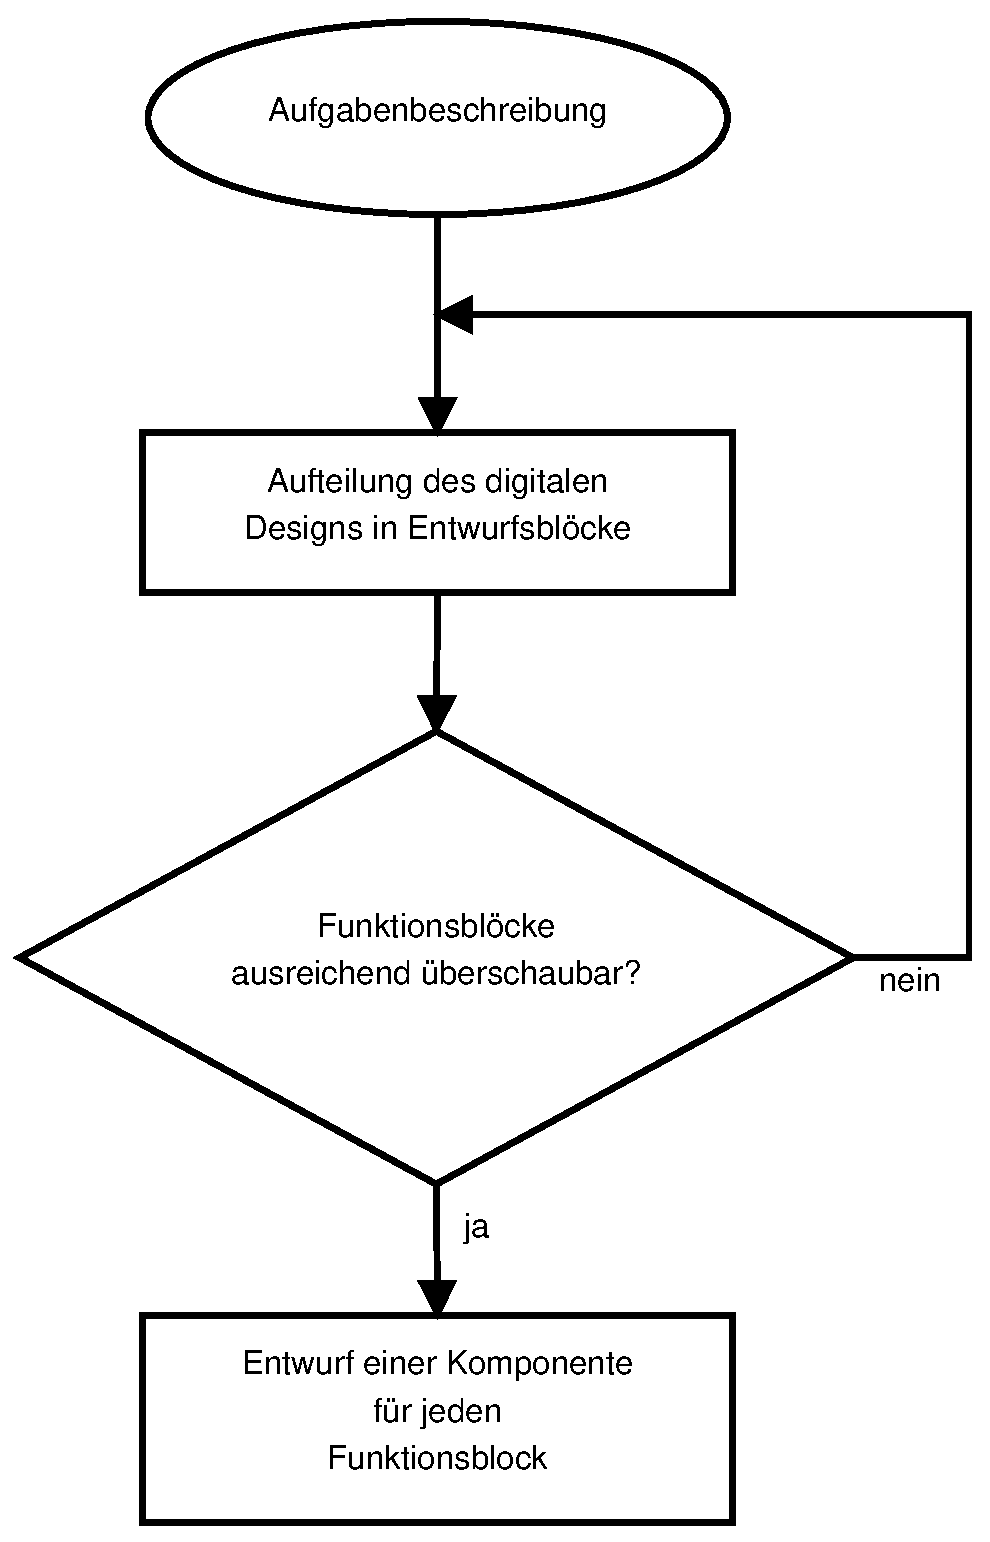
\includegraphics[width=0.25 \textwidth]{includes/Partitionierung.eps}
		\caption[Ablaufplan Partitionierung]{Ablaufplan zur Erstellung der Partitionierung eines digitalen Systems}
		\label{fig:Partitionierung}
	\end{center}
\end{figure}

\section{Struktureller Entwurf mit Komponenten}
\index{Struktureller Entwurf}
In diesem Abschnitt erläutern wir nun, wie der strukturelle Entwurf digitaler Systeme auf Basis vom
vorangegangen eingeführten hierarchisch aufgebauten \emph{entity/architecture}-Paaren realisiert wird.
In der übergeordneten Ebene wird dazu ein Strukturmodell formuliert, in dem diese Paare als 
Komponenten zu einer größeren Schaltung zusammengefaßt werden. Sie enthalten entweder die 
Verhaltensbeschreibungen digitaler Funktionen, oder sie bestehen wiederum aus Strukturbeschreibungen
einer hierarchisch niedrigeren Stufe. \cite{Reichardt}

Mit dem VHDL-Strukturbeschreibungsstil werden in einer Top-Entity die Signalkopplungen von mehreren
Komponenten in einer Architektur erzeugt. Jede Komponente bezieht sich somit auf eine untergeordnete
\emph{entity} mit mindestens einer dazugehörigen \emph{architecture}. In der Top-Entity sind deshalb 
nur die Schnittstellen der einzelnen Komponenten untereinander und zu Systemgrenzen Sichtbar und die
Top-Entity stellt somit eine textuelle Formulierung eines Blockschaltbildes dar. Welches von den
meisten Synthesewerkzeugen über eine Schaltplanausgabe automatisch erstellt werden kann.
\cite{Quartus-Manual} \cite{ISE-Manual} Mit diesem Ansatz wird dann ein Top-Down Entwurf verfolgt.

\vspace{10mm}
In der nun Vorliegenden strukturellen Architektur der Top-Entity werden die zu nutzenden Komponenten
zuerst mit ihren Schnittstellen deklariert und im Architekturrumpf instanziiert. In dieser Instanz
werden die Komponentenanschlüsse durch interne Koppelsignale bzw. durch Signale aus der
Schnittstellenliste der Top-Entity verdrahtet.
Zum leichteren Verständnis kann man sich Analog einen Hardwarebezug mit dem 
"`Board-Socket-Chip-Modell"'\cite{Perry} vorstellen. Hier repräsentiert die Top-Entity eine zu 
modelierende Platine (Board). Die Komponentendeklaration macht den IC-Typ mit seinen Anschlüßen 
bekannt. Wobei eine Komponenteninstanziierung dem Einlöten eines IC-Sockels (Socket) entspricht.
Mit der Konfiguration werden im letzten Schritt die IC-Sockel mit ICs bestückt, welche durch ihre 
speziellen \emph{entity/architecture}-Kombinationen die Funktionalität der Platine bestimmen.
\cite{Reichardt}

\section{Checkliste zum systematischen Systementwurf}
\index{Checkliste Systementwurf}
Basierend auf dem Daten-Steuerpfad-Modell lässt sich Folgende Checkliste aufstellen.
\begin{itemize}
	\item[1.] 	Identifizieren der Eingangs- und Ausgangssignale des Systems auf einem Blatt Papier
  				(Eingänge von links, Ausgänge nach rechts)
	\item[2.]	Analyse der Timing-Randbedingungen:
  				In welcher zeitlichen Reihenfolge müssen Eingangs- und Ausgangssignale eintreffen bzw. 
  				generiert werden, um die einzelnen Funktionen des Systems zu realisieren?
	\item[3.] 	Systempartitionierung des Datenpfads:
  				Welche Komponenten sind zur Lösung von Teilaufgaben geeignet?
	\item[4.] 	Analyse der Datenpfadkomponenten
  		\begin{itemize}
  			\item[4.1]	Blockdiagramm für den Datenpfad:
						Eine Liste mit erforderlichen lokalen Datenpfadsignalen.
			\item[4.2]	Welche Funktionsblöcke sind taksynchron und welche kombinatorisch?
			\item[4.3] 	Welche synchronen Komponenten benötigen einen synchronen/asynchronen Reset/Preset?
			\item[4.4] 	Analyse aller Datenpfadkomponenten:
						Welche Steuersignale sind für die verschiedenen Teilfunktionen erforderlich?
						Welche Statussignale werden erzeugt?
						Eintragung dieser in die Signalliste und ergänzen des Blockdiagramms.
			\item[4.5]	Ergänzung der Datenpfadkomponenten im Blockdiagramm durch eine entsprechende
						Abhängigkeitsnotation. 
  		\end{itemize}
	\item[5.]	Ergänzen des Blockdiagramms durch einen Zustandsautomaten für den Steuerpfad. Zunächst
				reicht ein Funktionsblock, welcher später im VDHL-Code durch zwei Prozeße modelliert wird.
	\item[5.1]	Welche externen und internen (lokalen) Datensignale steuern den Zustandsautomaten?
			 	Eintragen dieser in das Blockdiagramm und ergänzen der Signalliste.
	\item[5.2]	Sicherstellen das der Automat alle intern erforderlichen Steuersignale für den Datenpfad,
				sowie alle externen Steuersignale erzeugt.
	\item[5.3]	Festlegen der Automatenzustände (schriftlich):
				Wieviele Zustände?
				Welche Namen?
				Welche Funktion?
	\item[5.4]	Analysieren, welche Steuersignale Mealy- bzw. Moore-Charakter haben sollen.
	\item[5.5]	Zeichnen eines Zustandsdiagramms auf Basis der Datenpfadarchitektur und des zuvor 
				analysierten Timings für die verschiedenen Systemfunktionen. Sind abstrakte Bedingungen
				erforderlich, so ist dies ein Zeichen dafür, dass die Strukturierung des Datenpfads
				noch nicht detailiert genug ist.
	\item[5.6]	Prüfen der Vollständigkeit des Zustandsdiagramms:
		\begin{itemize}
			\item	Welches ist der Reset Zustand?
			\item 	Gibt es Zustände aus denen der Automat nicht mehr heraus kommt?
			\item 	Werden alle Kobinationen der Eingangssignale im Zustandsdiagramm berücksichtigt?
			\item 	Gibt es in allen Zuständen für alle Ausgangssignale eine Wertzuweisung?
					Welche Signalwerte eignen sich ggf. als Dafault im VHDL-Code?
		\end{itemize}
	 \item[6.]		Schreiben einer VHDL-entity unter Berücksichtigung aller im Blockdiagramm
	 				definierten Schnittstellensignale.
	 \item[7.]		Schreiben der architecture wie folg:
	 	\begin{itemize}
	 	  	\item[7.1]	Deklaration aller lokalen Signale der zuvor erstellten Signalliste. 
	 	  				Überlegungen, welcher Signaltyp verwendet werden soll.
	 	  	\item[7.2]	Deklaration jeweils eines Prozeßes und Entnahme aus dem Blockdiagramm, welche
	 	  				Datenpfadsignale erzeugt werden sollen.
	 	   	\item[7.3]	Erstellen zweier Prozeße für den Zustandsautomaten:
	 	   				hiervon muss ein Prozeß getaktet sein und einen in der Regel asynchronen
	 	   				Reset besitzen. Der andere Prozeß ist Kombinatorisch und erzeugt das
	 	   				Folgezustandsignal sowie in der Regel alle steuersignale.
	 	   	\item[7.4]	Ergänzen aller Prozeße durch ihre Empfindlichkeitslisten:
	 	   		\begin{itemize}
	 	   			\item	Bei kombinatorischen Prozeßen: Alle Eingangs- und Entscheidungssignale
	 	   			\item 	Bei taktsynchronen Prozeßen: Nur Systemtakt, sowie ggf. vorhandenen Reset
	 	   		\end{itemize}
	 	   	\item[7.5]	Ergänzen aller sequentieller Anweisungen, die die individuelle Funktion des
	 	   				Prozeßes beschreiben.
	 	\end{itemize}
\end{itemize}

\section{Umsetzung der Checkpunkte}
\index{Umsetzung Checkpunkte}
\texttt{Identifizieren der Eingangs- und Ausgangssignale des Systems auf einem Blatt Papier \\ (Eingänge von links, Ausgänge nach rechts)}

Aufgrund dieser Forderung ließ sich Folgende Grafik erstellen:
\begin{figure}[here]
	\begin{center}
		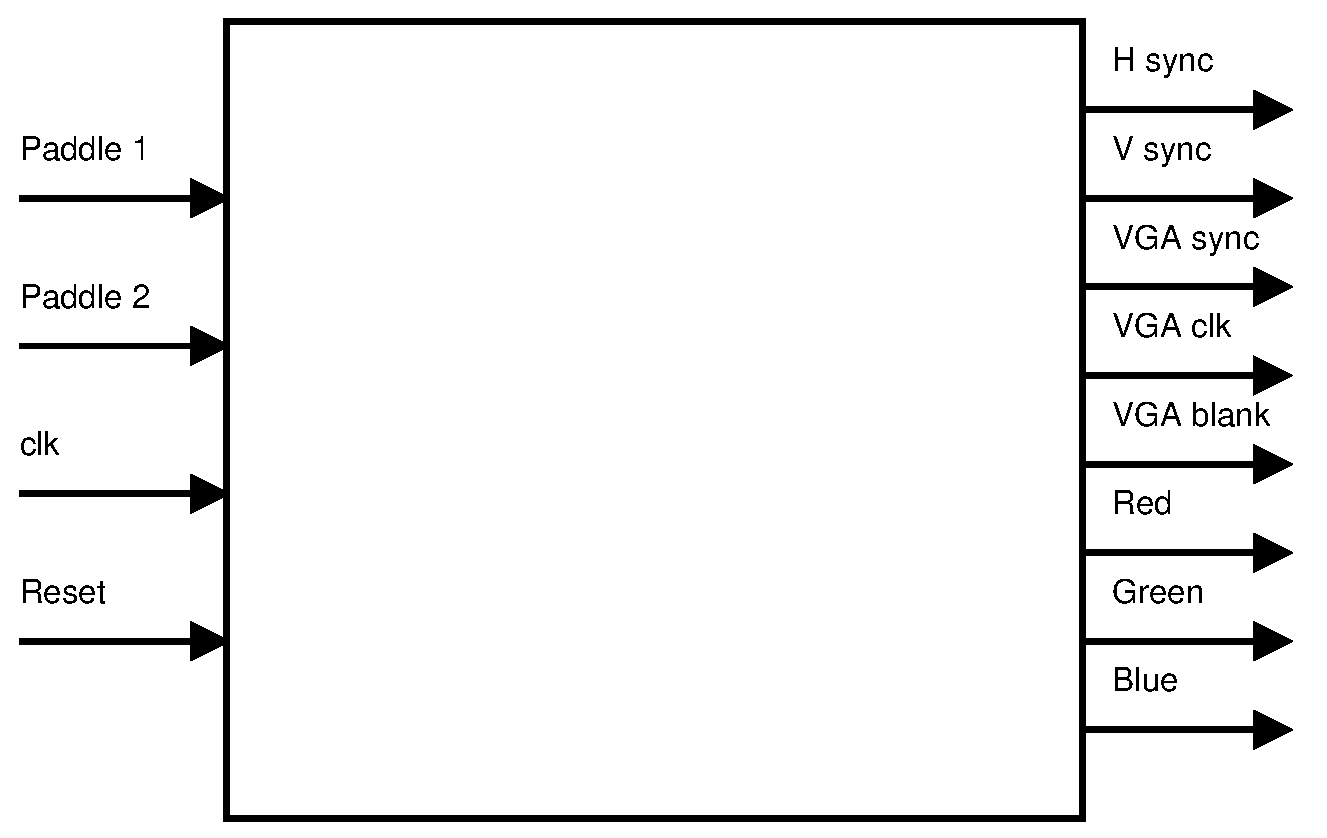
\includegraphics[width=0.65 \textwidth]{includes/TopEntity.eps}
		\caption[Eingangs- und Ausgangssignale des Systems]{Eingangs- und Ausgangssignale des Systems}
		\label{fig:Eingangs- und Ausgangssignale des Systems}
	\end{center}
\end{figure}

\newpage
Welche einen Taktgetriebenen Funktionsblock, mit asynchronen Reset und jeweils zwei (wie auch immer gearteten)
Eingangsvektoren für beide Bedienelemente darstellt. Als Ausgänge sind die Synchronisationsignale für Zeilen- und Spaltendarstellung, 
der eigentliche Pixeltakt (VGA clk), ein Ausgang zum deaktivieren der Anzeige (wird in der späteren Realisierung dazu verwendet um 
Bilddaten in den RAM zu schreiben) sowie die eigentlichen RGB-Signale definiert.
\vspace{7.5mm}

\texttt{Analyse der Timing-Randbedingungen:\\In welcher zeitlichen Reihenfolge müssen Eingangs- und Ausgangssignale
eintreffen bzw. generiert \\ werden, um die einzelnen Funktionen des Systems zu realisieren?}
\newline
Festzustellen war, dass beide Bedienelemente mit dem Systemtakt abzutasten sind und somit nicht von diesem abhängig sein durfen. 
Dies wurde in der späteren realisierung mit einer State-Machine realisiert. Die Timing Bedingungen zur Ansteuerung der VGA-Schnittstelle
sind zudem sehr komplex und es wird auf die weiterführende Literatur verwiesen.\cite{Hamblen}
\vspace{7.5mm}

\texttt{Systempartitionierung des Datenpfads:\\Welche Komponenten sind zur Lösung von Teilaufgaben geeignet?}
\newline
Zu erwähnen ist, dass wir die generierten Bildpunkte in einem eigens für diesen Zweck konzipierten RAM untergebracht haben (\emph{vga\_ram.vhd})
welcher hauptsächlich von zwei Elementen bearbeitet wird einem Game-Controller (\emph{game\_controller.vhd}) bzw. dem Video-Controller 
(\emph{video\_controller.vhd}). Des weiteren entsteht noch eine mit dem quartus Mega-Wizzard erstellte Phasen-Regelschleife, um einen Pixeltackt
nach gewählter Auflösung zu generieren.
z.B. 	25,75MHz bei 640x480 Pixeln @ 60Hz
		162,5MHz bei 1600x1200 Pixeln @ 60Hz.
Es wurden jeweils VESA zertifizierte Auflösungen gewählt, da diese von den meisten (in der Regel allen) Monitoren unterstützt werden und eine
Bildwiederholrate von 60Hz, da diese quasi Standard bei den von uns verwendeten TFT-Monitoren war.		
\vspace{7.5mm}



\newpage
\bibliography{library}
\listoffigures
\printindex
\end{document}
